%\documentstyle[epsf,twocolumn]{jarticle}       %LaTeX2.09仕様
%\documentclass[twocolumn]{jarticle}     %pLaTeX2e仕様
\documentclass[twocolumn]{jarticle} 

\AtBeginDvi{\special{pdf:mapfile texfonts.map}}

%一枚組だったら[twocolumn]関係のとこ消す

\setlength{\topmargin}{-45pt}
%\setlength{\oddsidemargin}{0cm} 
\setlength{\oddsidemargin}{-7.5mm}
%\setlength{\evensidemargin}{0cm} 
\setlength{\textheight}{24.1cm}
%setlength{\textheight}{25cm} 
\setlength{\textwidth}{18.0cm}
%\setlength{\textwidth}{172mm} 
\setlength{\columnsep}{11mm}

\def\baselinestretch{0.95}

\kanjiskip=.07zw plus.5pt minus.5pt

\usepackage{okumacro}
\usepackage[dvipdfm]{graphicx}
\usepackage{ascmac}
\usepackage{subcaption}
\usepackage{enumerate}
\usepackage{comment}
\usepackage{url}
\usepackage{multirow}
\usepackage{diagbox}
\usepackage{amssymb}
\usepackage{mathtools}
\usepackage{wrapfig}
\usepackage{graphicx}
\usepackage{float}
\usepackage{algorithmic}
\usepackage{amsmath}
\usepackage{algorithm}
\usepackage{lipsum}
\usepackage[jis2004]{otf}

\begin{document}
\twocolumn[
  \noindent
  \hspace{1em}

  2023 年 1 月 24 日情報工学実験 $\mathrm{I}\hspace{-1.2pt}\mathrm{I}$ 発表資料
  \hfill
  \ \  B3 西村昭賢 

  \vspace{2mm}
  \hrule
  \begin{center}
  {\Large \bf カードゲーム型対戦環境への深層強化学習の適用}
  \end{center}
  \hrule
  \vspace{3mm}
]

\section{はじめに}
近年, 人工知能に関する研究分野は目覚ましい発展を遂げており様々な分野に応用されている. その中でも人間の学習プロセスに近いとされる強化学習と深層学習を融合した深層強化学習が注目されている.\par
深層強化学習の応用先の 1 つとしてゲームがある.
特に将棋や囲碁といった, プレイヤーが意思決定をする段階でそれ以前の意思決定の過程がすべて把握可能な完全情報ゲームへの応用において成果が顕著である. 
最近では麻雀やポーカーのような, プレイヤーに与えられる情報が部分的である不完全情報ゲームへの応用も注目されている.
\par
そこで, 本研究では不完全情報ゲームであるトレーディングカードゲームを参考にカードゲーム型対戦環境を構築し, 構築環境へ深層強化学習手法を適用し学習済みエージェントの行動を観測した. 

\section{要素技術}

\subsection{OpenAI Gym}
OpenAI Gym \cite{OpenAIGym} は非営利企業 OpenAI が提供する強化学習のシミュレーション用ライブラリであり, 強化学習の環境として多くのゲームが登録されている. 提供されているインターフェースに沿って, エージェントの行動空間や状態空間, 報酬などを定義,実装することで自作の環境を登録し利用することができる. 様々な強化学習用ライブラリに対応しているため比較的容易に強化学習を試すことができる.


\subsection{Deep Q Network}
価値ベースの強化学習手法の 1 つ である Q 学習では実装の際に状態と行動をインデックスとする Q 値のテーブルを作成する. しかし状態空間や行動空間が高次元である, あるいは状態や行動が離散値ではなく連続値で表現される場合には Q テーブルのメモリ量は爆発してしまう. この問題を解決した技術が Deep Q Network (DQN) \cite{mnih2013atari} である.
 DQN ではニューラルネットワークを用いて, ある状態における行動ごとの Q 値を推定する.エージェントが経験した過去の体験を Replay Memory に一定期間保存しておき, 過去の経験をランダムにサンプリングして学習する Experience Replay や行動を決定する Q 値のネットワークと Q 値の学習を行うネットワークを分けることで Q 値の過大評価を防ぐ Fixed Target Network といった工夫により安定した学習を可能としている.

\section{カードゲーム型対戦環境の構築}
\subsection{トレーディングカードゲーム}
今回の実験で構築したカードゲーム型対戦環境は, Magic : The Gathering \footnote[1]{https://magic.wizards.com} といったトレーディングカードゲーム (Trading Card Game : TCG) を参考にした. TCG は 2 人のプレイヤーからなるゲームである. プレイヤーは先攻と後攻に分かれ, ターン制で進んでいく. 大きな特徴として将棋やチェスのように同じユニットを用いるのではなく, 事前に各プレイヤーの選択による異なるユニットからなるデッキを構築する点が挙げられる. 
ゲームタイトルごとに異なるが, 多くの場合相手プレイヤーのカードの 1 部分はプレイヤーから観測できない不完全情報ゲームである.

\subsection{構築環境}
実装したカードゲームのルールと用語を説明する.
ゲームは 2 人のプレイヤーからなり, プレイヤーは複数のカードからなるデッキを持つ. また, HP , マナといった 2 つの数値を持つ. 
プレイヤーは手札, 盤面と呼ばれるカードを保有する領域を持ち, ドローと呼ばれる操作でカードをデッキから手札に加える. また, プレイと呼ばれる操作でカードを手札から盤面に出す. プレイヤーがカードをプレイする際, 後述するカードのコスト分マナを消費する. また, デッキからカードが無くなった状態をデッキ切れと呼ぶ.  
今回の環境ではプレイヤーの HP は 20 , マナの上限値は初期値が 1 で最大値を 5 とした.
\par
カードはそれぞれ攻撃力と HP とコストの 3 つの数値を持つ. また, カードによっては特殊効果を持つものもある. 盤面にあるカードは対戦相手の盤面にあるカード, あるいは相手プレイヤーに攻撃することができる.ただし, 攻撃が可能となるのはカードがプレイされたターンの次のターンからになる. カードが攻撃を行う際には, 相手盤面に存在する攻撃対象のカードの HP, あるいは相手プレイヤーの HP へカードの持つ攻撃力分ダメージを与える. またカードへと攻撃する際には攻撃対象のカードが持つ攻撃力分, 攻撃するカードもダメージを受ける.
カードのHP が 0 になった, あるいは後述する手札と盤面の枚数制限を超えて盤面にプレイされた時はカードは破壊される. 破壊されたカードは捨て札となり盤面や手札から消え, ゲーム中には再出現しない. 
\subsection{ゲームフロー}
実装したゲームの流れを説明する.
\begin{enumerate}
  \small
  \setlength{\itemsep}{0cm} % 項目間
  \item ゲーム開始時に各プレイヤーは自身のデッキをシャッフル.
  \item デッキから初期手札としてカードを 5 枚ドロー. 
  \item 先攻プレイヤーは 1 ターン目のドローステップをスキップし行動.
  \item 後攻プレイヤーはカードを 1 枚ドローして行動.
  \item 2 ターン目以降は先攻プレイヤーもカードを 1 枚ドローしてから行動. 
  \item 4 , 5 の繰り返し. なお, ターンプレイヤーは行動前にマナを上限値まで回復. このときマナの上限値が 5 でなければ上限値を 1 増やしてから回復.
  \item どちらかのプレイヤーがデッキ切れになっている状態で,カードをドローしようとした, あるいはプレイヤー自身の HP が 0 となった場合はそのプレイヤーが敗北となりゲーム終了.
\end{enumerate}
\par
本構築環境では, 一般的な TCG と同様に先攻プレイヤーがカードの行動が早いため有利となる.そのため, 先攻の 1 ターン目のドローステップをスキップしている. 

\section{実験}
構築環境へ深層強化学習が適用できるか検証した.
深層強化学習手法として DQN を用いた. DQN を用いて構築環境において先攻のプレイヤーとして学習し, 学習済みのモデルを用いて 10000 回ゲームを実行して勝率を計算した. また, 学習が進んでいるかどうか判断するため学習時の獲得報酬の推移を記録し, 10000 回の実行結果から学習したエージェントがどのような戦略を構築したか, 人間から見て妥当な戦略かどうか考察した.

\subsection{対戦相手の行動ルーチン}

学習, 勝率計算の際は学習するプレイヤーの対戦相手を用意する必要がある.
Algorithm \ref{alg1} に今回の実験における対戦相手の手動で作成した行動ルーチンを示す.
\begin{figure}[t]
  \vspace{-0.3cm}
  \begin{algorithm}[H]
    \small
      \caption{
        対戦相手の行動ルーチン
        }
      \label{alg1}
      \begin{algorithmic}[1] 
      \STATE 盤面にカードを 1 枚プレイ
      \FOR{盤面のカード (プレイ順が古い方から)}
      \IF{敵の盤面に 1 回の攻撃で破壊できるカードがある}
      \STATE その攻撃対象を選んで攻撃
      \ELSE
      \IF{敵盤面の総攻撃力が自身の HP 以上}
      \STATE 敵盤面の最も攻撃力高いカードを攻撃
      \ELSE
      \STATE 敵プレイヤーを攻撃
      \ENDIF
      \ENDIF
      \ENDFOR
      \STATE ターンを終了
      \end{algorithmic}
  \end{algorithm}
  \vspace{-0.3cm}
  \end{figure}


\subsection{デッキ}
学習側,対戦相手ともに同じデッキを持つ.
表 \ref{table:deck} に, デッキに採用したカードの内容を示す. デッキは 表 \ref{table:deck} に示すカードを各 2 枚ずつ, 計 30 枚のカードから構成される. 
特殊効果は便宜上 2 字の単語で表しており, 具体的な効果は以下の通りである.

\begin{table}[t]
  \centering
  \small
  \caption{デッキに採用したカードの内容}
  \label{table:deck}
  \vspace{-0.3cm}
  \scalebox{0.90}[0.90]{
    \begin{tabular}{|c|c|c|c|c|}
      \hline
      ID & 攻撃力 & HP & コスト & 特殊効果 \\ \hline
      0 & 1 & 1 & 0 & 無し \\ \hline
      1 & 2 & 1 & 1 & 無し \\ \hline
      2 & 3 & 2 & 2 & 無し \\ \hline
      3 & 4 & 3 & 3 & 無し \\ \hline
      4 & 5 & 4 & 4 & 無し \\ \hline
      5 & 2 & 2 & 2 & 召喚 \\ \hline
      6 & 2 & 3 & 3 & 召喚 \\ \hline
      7 & 1 & 1 & 1 & 循環 \\ \hline
      8 & 1 & 3 & 2 & 循環 \\ \hline
      9 & 2 & 1 & 2 & 速攻 \\ \hline
      10 & 3 & 1 & 3 & 速攻 \\ \hline
      11 & 1 & 2 & 2 & 攻撃 \\ \hline
      12 & 2 & 3 & 3 & 攻撃 \\ \hline
      13 & 1 & 1 & 1 & 治癒 \\ \hline
      14 & 2 & 1 & 3 & 治癒 \\ \hline
      \end{tabular}
  }
  
\end{table}

  \begin{itemize}
  
  
  \setlength{\itemsep}{0cm} % 項目間
   \item 盤面に出したら (攻撃力 , HP) = ( 1 , 1 )のユニットを追加で盤面に出す (召喚)
   \item 盤面に出したら自プレイヤーの HP を 2 回復する (治癒)
   \item 盤面に出したら敵プレイヤーの HP を 2 減らす (攻撃)
   \item 盤面に出したら自プレイヤーは 1 枚カードをドローする (循環)
   \item 盤面に出たターンに攻撃できる (速攻)
  \end{itemize}


\subsection{状態空間と行動空間,報酬の定義}
強化学習では, エージェントの取りうる行動と観測できる状態の空間, 報酬を定義する必要がある. 
TCG ではドローやプレイ, カードの攻撃による破壊といった行動で盤面や手札の枚数が変化する場合があり, 各ステップ時点でプレイヤー取りうる行動の次元数が変わるため学習が困難である.\par
そのため本研究では予め手札と盤面の枚数の上限をそれぞれ 9 枚, 5 枚と定め, 手札と盤面に存在するカードに自盤面 1 というように番号をつけ, カードが存在しない場合は状態を 0 とすることで状態空間と行動空間を定義した. 表 \ref{table:state}, \ref{table:action} に状態空間, 行動空間の定義を示す.
なお, ドローやプレイといった操作でカードを追加し枚数の上限を超える場合には追加しようとしたカードを破壊する.
\par
reward は以下のように設定した.\par
\begin{itemize}
  \vspace{-0.3cm}
  \item 1 ステップ終了後 
  \begin{equation*}
    \vspace{-0.3cm}
   \mathrm{reward} = 0.0  
  \end{equation*}
  \item 1 エピソード終了後
  \begin{equation*}
    \vspace{-0.3cm}
    \mathrm{reward} = 
    \left\{
      \begin{aligned}
          1.0 \quad & (学習プレイヤーの勝利) \\
          -1.0 \quad & (敵プレイヤーの勝利) \\
      \end{aligned}
      \right.
  \end{equation*} 
  \vspace{-0.3cm}
\end{itemize}
\vspace{-0.3cm}



\begin{table}[t]
  \small
  \centering
  \caption{定義した状態空間}
  \label{table:state}
  \vspace{-0.3cm}
  \scalebox{0.85}[0.85]{
    \begin{tabular}{|c|c|c|c|}
      \hline
      状態説明                        & 次元数        & 最小値        & 最大値         \\ \hline \hline
      各プレイヤーの HP & 2 & 0 & 20 \\ \hline
      各プレイヤーの マナ & 2 & 0 & 5 \\ \hline
      \begin{tabular}{c}
        手札 1 $\sim$ 9 の\\HP , 攻撃力, コスト, 特殊効果
        \end{tabular}      & 36         & 0          & 5          \\
      \hline
      \begin{tabular}{c}
        自盤面 1 $\sim$ 5 の\\HP と攻撃力
      \end{tabular}     & 10         & 0          & 5 \\
      \hline
      \begin{tabular}{c}
        敵盤面 1 $\sim$ 5 の\\HP と攻撃力
      \end{tabular}     & 10         & 0          & 5 \\
      \hline
      \begin{tabular}{c}
        自盤面 1 $\sim$ 5 が\\攻撃可能かどうか
      \end{tabular} & 5          & 0          & 1  \\
      \hline
      \begin{tabular}{c}
        お互いのデッキの\\残り枚数
      \end{tabular}     & 2 & 0 & 30 \\
       \hline
      \end{tabular}
  }
  \end{table}

  \begin{table}[t]
    \centering
    \caption{定義した行動空間}
    \vspace{-0.3cm}
    \label{table:action}
    \scalebox{0.80}[0.85]{
      \begin{tabular}{|c|c|}
        \hline
        行動説明                          & 次元数        \\ \hline \hline
        手札 1 $\sim$ 9 を自盤面に出す             & 9          \\ \hline
        自盤面 1 が敵盤面 1 $\sim$ 5 に攻撃or敵プレイヤーに攻撃    & 6          \\ \hline
        自盤面 2 が敵盤面 1 $\sim$ 5 に攻撃or敵プレイヤーに攻撃    & 6          \\ \hline
        自盤面 3 が敵盤面 1 $\sim$ 5 に攻撃or敵プレイヤーに攻撃    & 6          \\ \hline
        自盤面 4 が敵盤面 1 $\sim$ 5 に攻撃or敵プレイヤーに攻撃    & 6          \\ \hline
        自盤面 5 が敵盤面 1 $\sim$ 5 に攻撃or敵プレイヤーに攻撃    & 6          \\ \hline
        ターンエンド & 1 \\ \hline
        \end{tabular}
    }
    \end{table}
  
  \subsection{DQN のパラメータ}
  表 \ref{table:dqnparam} に実験で用いた DQN のパラメータを示す. \par
  また, ε-greedy において $\epsilon$ は ( \ref{epsilon} ) 式に従って, $\mathrm{\epsilon_{max}}$ から $\mathrm{\epsilon_{min}}$ へと指数関数的に減少する. 
  \begin{equation}
    \vspace{-0.3cm}
    \small
    \label{epsilon}
    \epsilon = \mathrm{max}(\mathrm{\epsilon_{min}} \: , \: \mathrm{\epsilon_{min}} + (\mathrm{\epsilon_{max} - \epsilon_{min}}) \exp(- \frac{stepcount}{\mathrm{\epsilon_{decay}}}))
  \end{equation}
  なお, 本実験では $\mathrm{\epsilon_{max}} = 1.0, \mathrm{\epsilon_{min}} = 0.1, \mathrm{\epsilon_{decay}} = 50.0$ とした.  

  \begin{table}[t]
    \centering
    \caption{DQNのパラメータ}
    \vspace{-0.3cm}
    \label{table:dqnparam}
    \scalebox{0.80}[0.80]{
      \begin{tabular}{|c|c|}
        \hline
        パラメータ名 & 値 \\ \hline \hline
        割引率 $\gamma$ & 0.99 \\ \hline     
        全結合層の活性化関数             & ReLU     \\ \hline
        全結合層の次元                & 64       \\ \hline
        最適化アルゴリズム              & Adam     \\ \hline
        方策                 & ε-greedy \\ \hline
        Target Network 更新重み              & 0.5     \\ \hline
        Exprience Memory 開始ステップ数 & $1.0 \times 10^5$ \\ \hline
        学習ステップ数 &  $1.0 \times 10^6$ \\ \hline
        \end{tabular}
    }
    \end{table}
  

\section{結果と考察}
表 \ref{table:result} に実験結果を示す. なお,ベースラインとして対戦相手と同じ戦略を持つプレイヤー, 表 \ref{table:action} の行動空間に沿ってランダムに行動するプレイヤーを先攻に配置して 10000 回対戦し勝率を計算した結果を示している.\par 
\begin{table}[t]
  \centering
  \caption{実験結果}
  \vspace{-0.3cm}
  \label{table:result}
  \scalebox{0.80}[0.80]{
    \begin{tabular}{|c|c|}
      \hline
      手法 & 勝率 \\ \hline \hline
      DQN & \textbf{0.9739} \\ \hline
      対戦相手と同じ戦略 & 0.5089 \\ \hline     
      ランダム & 0.3155 \\ \hline

      \end{tabular}
  }
  \end{table}
  DQN で学習したエージェントは, 9 割 7 分とベースラインと比べて遥かに高い勝率を残している. また,  図 \ref{fig:DQNresult} に DQN における学習時の平均獲得報酬の推移を示す. 図 \ref{fig:DQNresult}  において縦軸は reward, 横軸はエピソード数であり, 図中の緑点は 学習時の 100 エピソードにおける平均獲得報酬を表し, 薄緑の領域は標準偏差を表す.
  およそ 2000 エピソード学習した段階で獲得報酬が大きく上昇し, それ以降は学習が安定している. 
  また, 学習済みエージェントにおける 10000 回の対戦のログからエージェントがどのような戦略を構築したか, 人間から見て妥当かどうか検証した.  ( \ref{epsilon} ) 式から, 学習序盤はランダムに探索をしているため学習済みエージェントの対戦ログの比較対象としてランダムに行動するプレイヤーの対戦ログを用いる.
  \par
  表 \ref{table:actioncount} に 10000 回の対戦においてランダムに行動するプレイヤーがとった行動の総数と, DQN で学習済みエージェントがとった行動の総数を示している. 
  表 \ref{table:actioncount} から行動の総数が学習済みエージェントでは全体的に減少しており, 相手プレイヤーに直接攻撃するといった行動が多く取られている. このことから, DQN では TCG における先攻の優位性を生かして相手プレイヤーに攻撃する戦略が最適だと学習されたといえる. 
  また, ランダムに行動するプレイヤーが最も多く選択していたターンエンドは, DQN では 2 番目まで下がっている. これは, まだカードがプレイできる状態でターンエンドするといった無駄なターンエンドをする傾向が減っていると言える. これは人間から見ても妥当な行動といえる.\par
  また,  表 \ref{table:cardcount} には 10000 回の対戦において各カードがプレイされた回数である. 表 \ref{table:cardcount} において, DQN で学習済のエージェントは 0, 1, 2 コストのカードに関してはコストが小さいカードほど多くプレイされている. これは行動の総数で考察したように無駄なターンエンドは損であると学習し, マナを余らせること無くカードを盤面にプレイできていると考えられる. 
  また, 4 コストの ID 4 のカードが 3 コストの ID 6, 10, 14 に比べて多くプレイされている. ID 4 のカードは HP が唯一 4 となるカードであり対戦相手は, Algorithm \ref{alg1} に従うため, 対戦相手は ID 3, 4 のカードを盤面に出さなければ ID 4 のカードは破壊されることがない. また攻撃力も 5 と全カード中最大であるためこの実験条件においてはカードパワーが高いカードである. そのため ID 4 のカードを盤面に出すことが得であると学習して全カード中コストが最大であるにもかかわらず, 3 コストの 3 枚より優先して盤面に出されている. この行動も妥当である.

  \begin{table}[t]
    \centering
    \caption{選択された総数が多い行動上位 5 つ (降順)}
    \vspace{-0.3cm}
    \label{table:actioncount}
    \scalebox{0.68}[0.70]{
      \begin{tabular}{|cc|cc|}
        \hline
        \multicolumn{2}{|c|}{ランダム}      & \multicolumn{2}{c|}{DQN}       \\ \hline
        \multicolumn{1}{|c|}{行動説明} & 総数 & \multicolumn{1}{l|}{行動説明} & 総数 \\ \hline \hline
        \multicolumn{1}{|c|}{ターンエンド}    & 119543  & \multicolumn{1}{l|}{手札 1 を盤面にプレイ}    & 76955  \\ \hline
        \multicolumn{1}{|c|}{手札 1 を盤面にプレイ}    & 68762  & \multicolumn{1}{l|}{ターンエンド}    & 61799  \\ \hline
        \multicolumn{1}{|c|}{手札 2 を盤面にプレイ}    & 45215  & \multicolumn{1}{l|}{盤面 1 で相手プレイヤーに攻撃}    & 52531  \\ \hline
        \multicolumn{1}{|c|}{盤面 1 で相手プレイヤーに攻撃}    & 29951  & \multicolumn{1}{l|}{盤面 2 で相手プレイヤーに攻撃}    & 27875  \\ \hline
        \multicolumn{1}{|c|}{盤面 1 で敵盤面 1 を攻撃}    & 24720  & \multicolumn{1}{l|}{手札 2 を盤面にプレイ}    & 15191  \\ \hline
        \end{tabular}
    }
  \end{table}

  \begin{table}[t]
    \centering
    \caption{各カードが盤面にプレイされた総数 (降順)}
    \vspace{-0.3cm}
    \label{table:cardcount}
    \scalebox{0.75}[0.65]{
      \begin{tabular}{|ll|ll|}
        \hline
        \multicolumn{2}{|c|}{ランダム}       & \multicolumn{2}{c|}{DQN}       \\ \hline
        \multicolumn{1}{|l|}{ID} & 総数    & \multicolumn{1}{l|}{ID} & 総数   \\ \hline \hline
        \multicolumn{1}{|l|}{0}  & 12208 & \multicolumn{1}{l|}{0}  & 8463 \\ \hline
        \multicolumn{1}{|l|}{1}  & 12015 & \multicolumn{1}{l|}{13} & 8069 \\ \hline
        \multicolumn{1}{|l|}{9}  & 11818 & \multicolumn{1}{l|}{1}  & 7971 \\ \hline
        \multicolumn{1}{|l|}{11} & 11791 & \multicolumn{1}{l|}{7}  & 7845 \\ \hline
        \multicolumn{1}{|l|}{13} & 11751 & \multicolumn{1}{l|}{11} & 7693 \\ \hline
        \multicolumn{1}{|l|}{2}  & 11674 & \multicolumn{1}{l|}{2}  & 7672 \\ \hline
        \multicolumn{1}{|l|}{7}  & 11513 & \multicolumn{1}{l|}{5}  & 7663 \\ \hline
        \multicolumn{1}{|l|}{5}  & 11459 & \multicolumn{1}{l|}{9}  & 7483 \\ \hline
        \multicolumn{1}{|l|}{10} & 11345 & \multicolumn{1}{l|}{8}  & 7372 \\ \hline
        \multicolumn{1}{|l|}{12} & 11317 & \multicolumn{1}{l|}{3}  & 6910 \\ \hline
        \multicolumn{1}{|l|}{8}  & 11158 & \multicolumn{1}{l|}{12} & 6876 \\ \hline
        \multicolumn{1}{|l|}{3}  & 11091 & \multicolumn{1}{l|}{4}  & 6862 \\ \hline
        \multicolumn{1}{|l|}{14} & 11057 & \multicolumn{1}{l|}{6}  & 6720 \\ \hline
        \multicolumn{1}{|l|}{6}  & 10884 & \multicolumn{1}{l|}{10} & 6630 \\ \hline
        \multicolumn{1}{|l|}{4}  & 10742 & \multicolumn{1}{l|}{14} & 6567 \\ \hline
        \end{tabular}
    }
    \end{table}


\section{まとめと今後の課題}
今回の実験では TCG を参考としたカードゲーム型対戦環境を構築し, 構築環境へ DQN を適用した. 構築環境において DQN と高い勝率を記録するエージェントを作成することができ, 学習が進んでいくにつれてエージェントが高い報酬を得るよう学習していることが実験により確認できた. また, 学習によりエージェントが構築した戦略を確認し, 人間から見ても合理的な戦略を構築していたことが確認できた.
\par
今回の環境では最適解が相手プレイヤーを直接攻撃する戦略であり, 盤面にあるカードへの攻撃処理が学習の際に無駄と判断された. そのため, 実質手札から最もダメージが期待できるカードを出すだけになってしまい, 盤面における戦略性が無くなってしまった. デッキの構成や対戦相手の戦略, 新たな特殊効果の追加などでより複雑で戦略性の高いカードゲーム型対戦環境を構築することが今後の課題として挙げられる.

\begin{figure}[t]
  \centering
  \small
  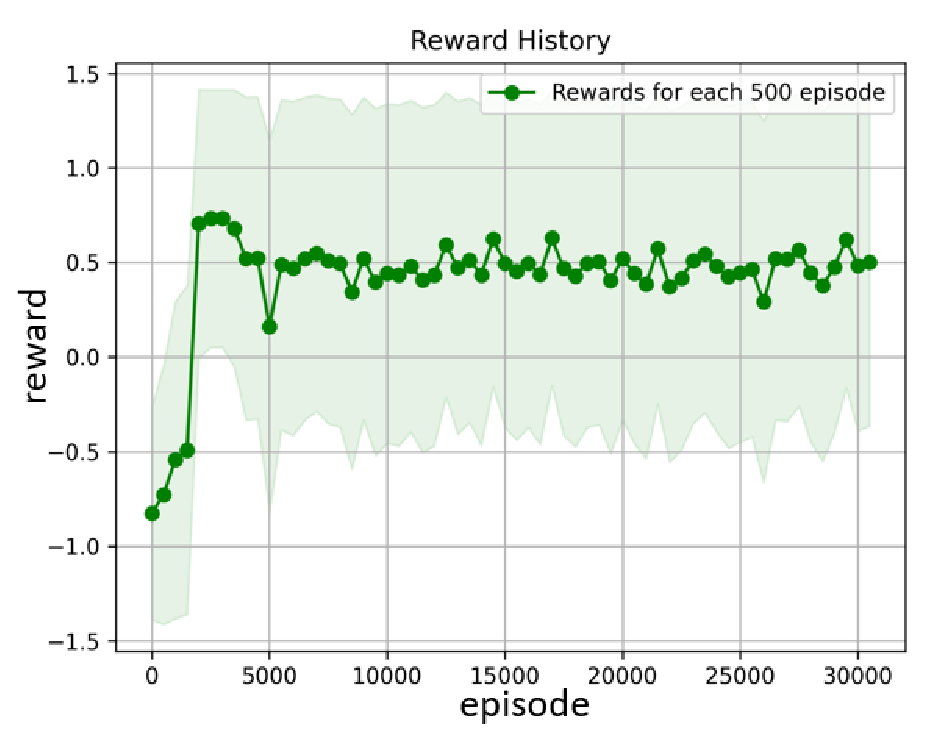
\includegraphics[width=73.5mm]{assets/graph.eps}
  \caption{DQN における平均獲得報酬の推移}
  \label{fig:DQNresult}
\end{figure}




%index.bibはtexファイルと同階層に置く
%ちゃんと\citeしないと表示されない(1敗)
\bibliography{index.bib}
\bibliographystyle{junsrt}

\end{document}